\documentclass[12pt]{article}
\usepackage[square, numbers, comma, sort&compress]{natbib} 
\usepackage{graphicx}
\begin{document}
\title{Nanoparticle Modeller for Martini - \emph{Martini-PyNP} - A Proposal}
\author{Sang Young Noh}
\date{\today}
\maketitle
\section{Introduction}
The introduction of software frameworks when constructing biomolecular systems and phase systems has revolutionized the pace of research in the
molecular simulation field. This is due to the ease of entry with the python programming language, as well as the use of molecular template contruction software,
such as moltemplate (for general use) \cite{Moltemplate}, insane (for the use of Martini and bilayers/proteins) \cite{INSANE}. Nanoparticle structures (NPs), on the other hand, have seen a number of software that have seen use such as nanomodeler \cite{Nanomodeller}. The case of nanomodeler and its use highlights the importance but also the difficulty of creating a general software that can manage the
construction of structures. As highlighted by Franco-Ulloa \emph{et al}, there are two main reasons for this:
\begin{itemize}
\item Construct complex 3D models of the inner metal core and outer layer of organic ligands.
\item Correctly assign force-field parameters to these composite systems.
\end{itemize} 
Other factors that inhibit the ease of construction of such software is that NPs can occur with several sizes and morphology, for example the carbon nanotube being a classical
model which should be taken into account to create a general software. 
\newline
\newline
Recent developments in existing software packaged have helped to make this goal closer towards being substatial. MDAnalysis is one of the de-factor molecular packages that
is avaliable for manipulating PDB/GRO/XYZ molecular topologies, as well as TRR/DCD/XTC binary trajectories from simulation files to analyze according to how one wants to look at the simulation. 
The most recent version, MDAnalysis-1.0.1, added new functionalities, of structural analysis but especially a cross-link compatibility with SMILES strings of molecules, which in turn
allows it to utilize the RDKit library, which is already a very-well established chemiinformatics library. From the introduction of the RDKit conversion functionality in MDAnalysis (more information here - https://www.mdanalysis.org/2020/08/29/gsoc-report-cbouy/) the potential for simply inputting a smiles string to construct a ligand on the nanoparticle has been a potential. RDKit is convenient as it can detect what ligands is not suitable due to their unrealistic nature.
\newline
\newline
Another advantage with the RDkit infrastructure is the way aromatic atoms can be identified. Following the procedures by Alessandri \emph{et al} \cite{SmallMolecules}, we already know that with MARTINI3, aromatic and non-aromatic atomic moeities can have significantly different coarse-graining procedures, where instead of a normal 4-to-1 conversion from atomistic to coarse-grained, the mapping may require a 3-to-1 or even a 2-to-1 mapping. Previous approaches to NP construction include those that were done by Monticelli \cite{Fullerene} which involved the use of rigid  
\newline
\newline
\newline
\newline
\section{Proposed Code Workflow}
\begin{figure} %this figure will be at the right
  \centering
  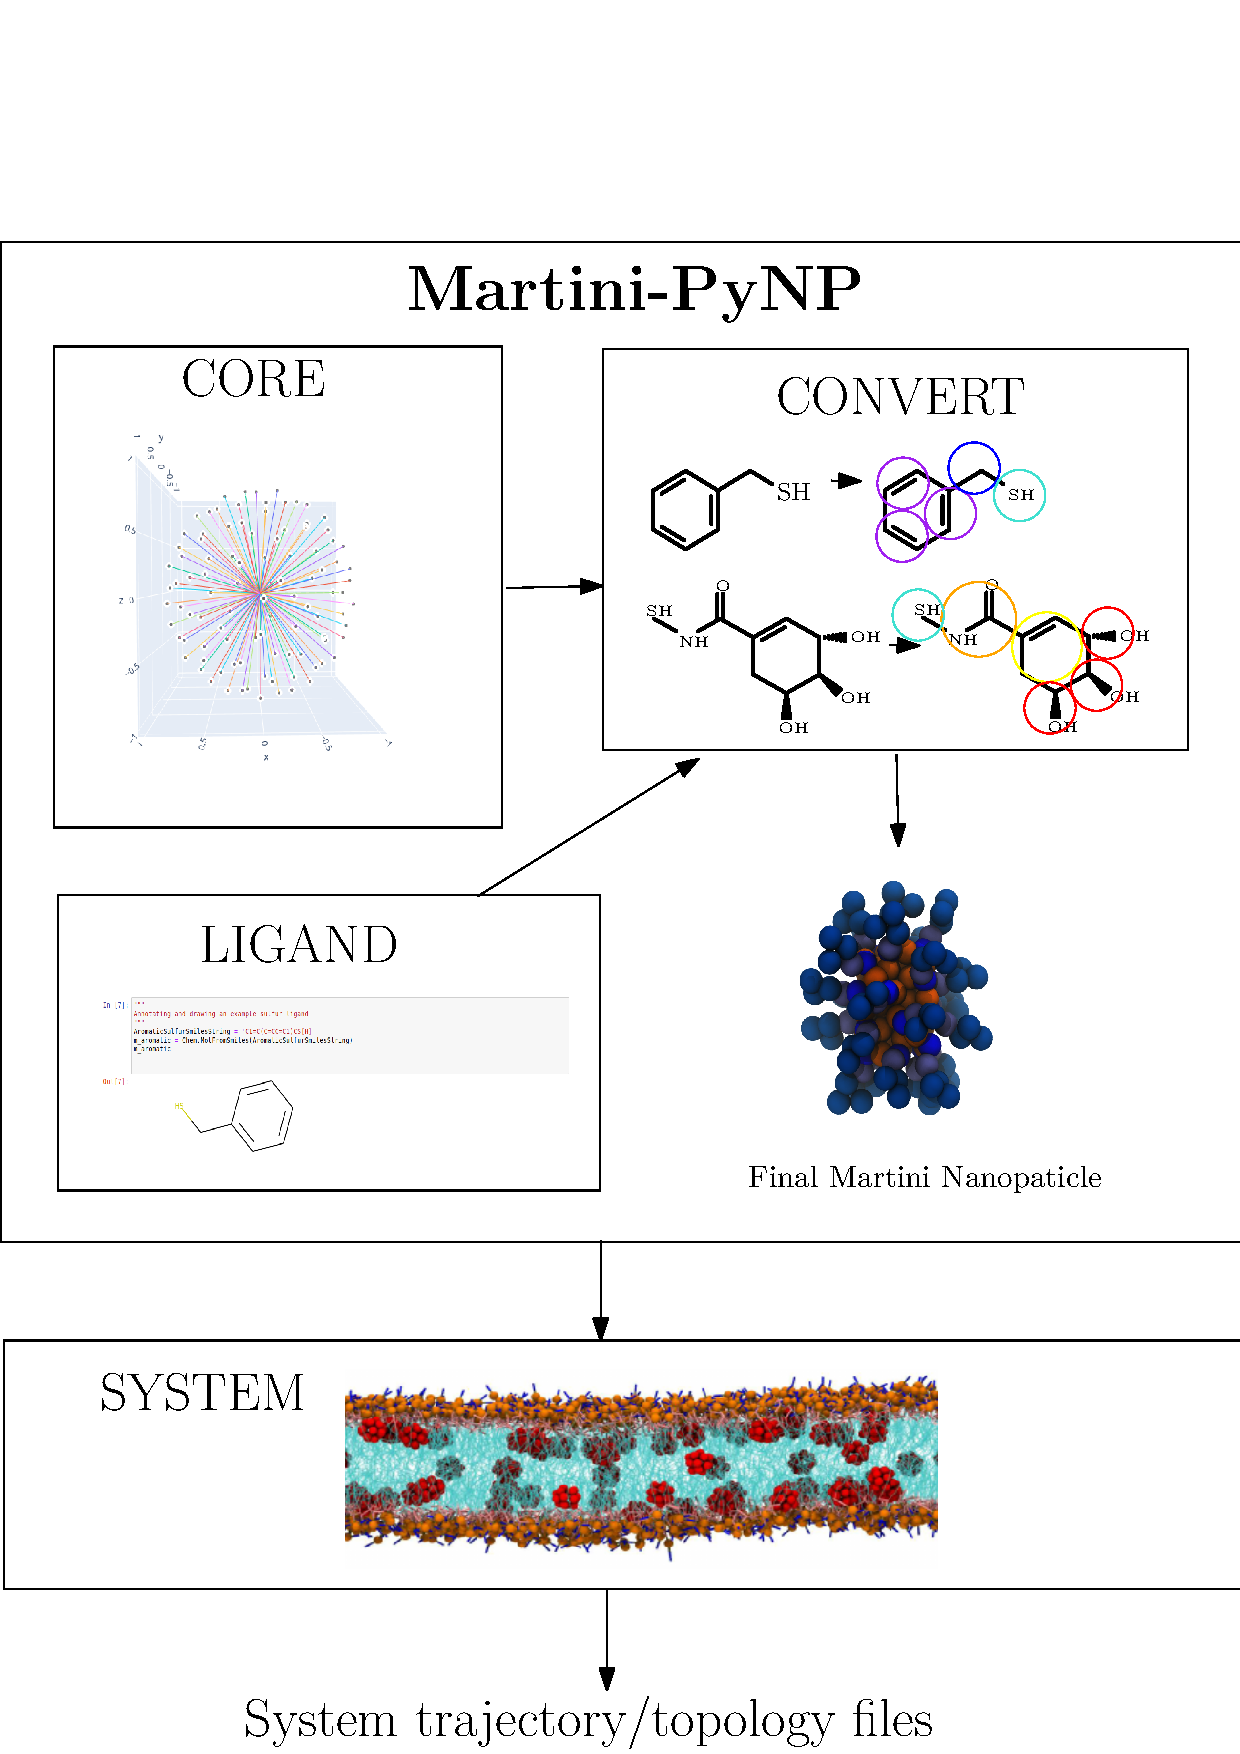
\includegraphics[scale=0.4]{schema.pdf}
  \caption{General flowchart for how the NP construction takes place. The SYSTEM module has been omitted from the figure, but will be added later}
\end{figure}
The code workflow is primarily developed in Python, to leverage the wide range of molecular structure libraries already avaliable. Here, we have divided the
primary construction code of Martini-PyNP into 4 main modules: 
\begin{itemize}
\item CORE
\item LIGAND
\item CONNECT
\item SYSTEM 
\end{itemize}
The CORE module handles the central sphere/nanotube construction, the LIGAND module would handle the construction of the ligand(s), to remove/parse
the structure so that unrealistic steric hindrances do not cause the breakdown of the simulation. The CONNECT module handles the attachment of the ligands
onto the NP surface - where one can determine one wants to make the ligands into a striped/janus/random mix type, or a custom surface pattern that one can define. Also,
the conversion of this system to the MARTINI 3 morphology would be done in this module. The SYSTEM deals with the construction of sample systems that the NP(s) can be placed, whether it be a lipid bilayer or a solvent system. 
\section{Reference Links}
\begin{itemize}
\item https://cedric.bouysset.net/blog/2020/06/18/gsoc-rdkit-to-universe - Rdkit tutorial
\item https://www.sciencedirect.com/science/article/pii/S0022283621000358 - Moltemplate literature
\item https://pubs.acs.org/doi/10.1021/acs.jctc.8b01304 - Nanomodeler
\item https://pubs.acs.org/doi/abs/10.1021/jacs.6b11717 - Heterojunction morphologies 
\item http://cgmartini.nl/index.php/martini-3-0 - Martini 3 parameters
\item https://chemrxiv.org/engage/chemrxiv/article-details/60f3ea062b910135237380eb - Mapping of the ligands to specific beads of martini
\item https://cedric.bouysset.net/blog/2020/08/07/rdkit-interoperability - Information on interoperatbility of the RDKit library and the MDAnalysis library
\item http://www.cgmartini.nl/index.php/example-applications2/35-downloads/exampleapplications/193-f16 - Fullerene models in Martini
\end{itemize}

\bibliographystyle{abbrv}
\bibliography{Documentation}
\end{document}
